%% LyX 2.3.5-1 created this file.  For more info, see http://www.lyx.org/.
%% Do not edit unless you really know what you are doing.
\documentclass[twocolumn,english]{extarticle}
\usepackage[LGR,T1]{fontenc}
\usepackage[utf8]{luainputenc}
\usepackage{color}
\usepackage{textcomp}
\usepackage{amsmath}
\usepackage{amsthm}
\usepackage{amssymb}
\usepackage{graphicx}
\usepackage{esint}

\makeatletter

%%%%%%%%%%%%%%%%%%%%%%%%%%%%%% LyX specific LaTeX commands.
\DeclareRobustCommand{\greektext}{%
  \fontencoding{LGR}\selectfont\def\encodingdefault{LGR}}
\DeclareRobustCommand{\textgreek}[1]{\leavevmode{\greektext #1}}
\ProvideTextCommand{\~}{LGR}[1]{\char126#1}


%%%%%%%%%%%%%%%%%%%%%%%%%%%%%% Textclass specific LaTeX commands.
\numberwithin{equation}{section}
\numberwithin{figure}{section}

%%%%%%%%%%%%%%%%%%%%%%%%%%%%%% User specified LaTeX commands.
\usepackage{preprint/authblk}

\AtBeginDocument{
  \def\labelitemi{\normalfont\bfseries{--}}
}

\makeatother

\usepackage{babel}
\begin{document}
\title{Direct Calculation of Double Counting Rate for Neutron Multiplicity
Methods}
\author{Wilfried Monange \thanks{Institut of Radioprotection and Nuclear Safety} \and Grégory Caplin \thanks{ORANO at IRSN when the work was prepared} \and Olivier Jacquet \thanks{Subcontractor}}
\maketitle

\section{Introduction}

Neutron density in nuclear system is subject to fluctuations that
arise from a random process. For sub-critical systems with large number
of neutrons these fluctuations are usually small enough so that the
well known Boltzmann equation is valid and the system is correctly
described by the mean quantities. On the other hand, a law neutron
density implies predominantly neutron fluctuations over average values
and other techniques must be used to describe the neutron population.
Among them, the Neutron Multiplicity Counting (NMC) \cite{NMC Robba}
focus on correlated time neutrons (i.e. neutrons belonging to the
same fission chain) detections for sub-critical system \emph{via}
the use of mean single count rate (i.e. mean count rate of detection),
double count rate (i.e. mean count rate of time correlated pairs of
detections), triple (i.e. mean count rate of time correlated triples
of detections), etc. In this way NMC is based on higher-order moment
of the counting distribution.

Usually NMC values obtained by simulation are calculated with algorithms
very similar to those used with real detectors and therefore only
make use of detection times. Depending on the simulation tools, the
calculation of these values is performed directly inside the simulation
code or outside \emph{via} output files (List-mode like) and post-processing
programs. This approach is referred here to as the \emph{analog method.}
As this method require exact simulation of the transport of neutrons,
i.e. analog calculation, ordinary Monte Carlo techniques for variance
reduction (Russian roulette, splitting etc.), which only preserve
first order moment (mean quantities), can no more be use.

As a consequence and although dating back to the early nuclear era,
the use and study of NMC techniques has been for many years limited
by the performance of computers that struggled to simulate the entire
neutron population of an experiment. Thanks to modern computers a
number of barriers have been raised and these techniques are now regularly
used for the reactivity assessment of low power or ADS reactors, non-destructive
assay of special nuclear material and for sub-critical benchmarks.

However, NMC simulations can still be very CPU time consuming under
certain circumstances such as configurations with huge calculation
time for neutron transport or when NMC values with large time scale
are required. To solve this problem, variance reduction techniques
applied to neutron noise techniques have been developed \cite{Szieberth}.
This paper proposes another approach based on the use of analog simulation
tools taking advantage of an additional information provided by the
code : the fission chain identifier (or history identifier) to which
a detection belongs. This information makes it possible to identify
the correlated detections, i.e. resulting from the same fission chain.
This approach will be referred to the \emph{direct method. }The word
``direct'' refer to the direct identification of correlated detections.
This paper will focus on the calculation of the single counting rate,
the double counting rate and the so called Feynman Y curve~\cite{Feynman}.

The map of this paper is as follows. The first part recall the \emph{analog
method} methodology, then the theory of the direct method is described
and is applied to a real experiment in the last part.

\section{Analog method}

The calculation of NMC values has been extensively described in the
literature \cite{Uhrig,Hutchinson1}. This section recall the basis
with the Hage-Cifarelli formalism \cite{Cifarelli} in order to introduce
the next section. During an NMC simulation neutron detections are
time-tagged and stored into a file, this create the so called \emph{signal}.
Next, the post processing divide this \emph{signal} into equal samples
of width $\tau$. For each of them the number of events are counted
and binned into a histogram called the Feynman histogram. From these
the $c_{k}$values representing the number of times $k$ detections
are found in samples are deduced. This can be repeated for multiple
samples widths resulting in multiple Feynman histograms. The NMC values
are finally calculated with the following formulas:

\[
m_{1}(\tau)=\frac{\underset{k}{\sum}k\,c_{k}(\tau)}{\underset{k}{\sum}c_{k}(\tau)}
\]
\[
m_{2}(\tau)=\frac{1}{2}\frac{\underset{k}{\sum}k(k-1)c_{k}(\tau)}{\underset{k}{\sum}c_{k}(\tau)}
\]

\[
Y_{1}(\tau)=\frac{m_{1}(\tau)}{\tau}
\]
\[
Y_{2}(\tau)=\frac{1}{\tau}\left(m_{2}(\tau)-\frac{1}{2}m_{1}(\tau)^{2}\right)
\]
\[
Y(\tau)=2\times\frac{Y_{2}(\tau)}{Y_{1}(\tau)}
\]

Where $Y_{1}$ and $Y_{2}$ stand for the single and double counting
rates for samples of width $\tau$, $Y$ is the Feynman-Y value, $m_{1}$
and $m_{2}$ being the first two reduced factorial moments as expressed
in the Hage-Cifarelli formalism.

As $\tau$ tends to infinity, $Y_{1}(\tau)$, $Y_{2}(\tau)$ and $Y(\tau)$
tend to their respective asymptotic values named $R_{1}$, $R_{2}$
and $Y_{\infty}$. This reflects the fact that as $\tau$ increase,
all detections from the same fission chain tend to be taken into account
and further increase of $\tau$ has negligible or no influence. In
order to reduce uncertainties the number of samples used must be large.
If one want to cover delayed neutron, large samples are required and
the simulated signal can required unacceptable CPU time or experiment
duration. As a consequence $R_{1}$, $R_{2}$ and $Y_{\infty}$ are
in practice estimated throw formulas depending of $Y_{1}(\tau)$,
$Y_{2}(\tau)$ and $Y(\tau)$  making these values dependent of both
the samples width (i.e. $R_{1}(\tau)$, $R_{2}(\tau)$ and $Y_{\infty}(\tau)$)
and the underlying theory. Note that for these values to be meaningful
and usable for other measures (calculation of total multiplication
for instance), the experiment must be in a steady state, i.e. the
power remains constant over time.

\section{Direct method}

Let $S$ be the mean rate of source events (i.e. the mean number of
histories per time unit) and $p_{N}$~the probability for an history
to create $N$ detections. Both values comes from simulation results.
In particular, the association of each detection with the fission
chain identifier makes it possible to calculate the $p_{N}$~quantity.
That being said, for a stationary process the mean rate of detections
from histories creating $N$ detections is $S\cdot p_{N}\cdot C_{N}^{1}$
where the letter $C$ denote the binomial coefficient. Summing over
all possible numbers of detections gives the single rate of detections:
\begin{equation}
\mathring{Y}_{1}=S\sum_{N=1}^{\infty}p_{N}\cdot C_{N}^{1}\label{eq:y1_final}
\end{equation}

In this formula as well as for the following, the circle denotes values
calculated using the \emph{direct method}. One may note that $\mathring{Y}_{1}$
does not depend on any samples width values and thus it is equal to
its asymptotic value $\mathring{R}_{1}$. To be consistent with formulas
presented in section 2 the expected number of detections per samples
$\mathring{m}_{1}$~is defined as $\mathring{Y}_{1}\,\tau$.

The same approach is then applied for the double counting rate. Considering
the mean rate of correlated pairs triggered by the \emph{ith} detection
of histories creating $N$ detections is $S\cdot p_{N}\cdot C_{N-i}^{1}$,
the mean double counting rate created by histories having $N$ detections
is equal to:
\[
S\cdot p_{N}\sum_{i=1}^{N-1}C_{N-i}^{1}=S\cdot p_{N}\cdot C_{N}^{2}
\]

Taking into account all histories with any number of detections gives
the asymptotic mean double counting rate $\mathring{R}_{2}$: 
\begin{equation}
\mathring{R}_{2}=S\sum_{N=2}^{\infty}p_{N}\cdot C_{N}^{2}\label{eq:r2_final}
\end{equation}

Contrary to the \emph{analog method,} simulation results give directly
access to the asymptotic double counting rate without the need of
intermediate formulas. As a consequence $\mathring{R}_{2}$~do not
depends of neither $\tau$ or an underlying theory but only on the
number of simulated histories.

We are now interested in the calculation of the non-asymptotic value
of $\mathring{R}_{2}$, i.e. $\mathring{Y}_{2}(\tau)$. Let's consider
a first detection in the time range $\left[t_{1},t_{1}+dt_{1}\right]$
and a second one inside $\left[t_{2},t_{2}+dt_{2}\right]$ with $t_{1}<t_{2}$,
the average number of correlated pairs of detections $S_{r}$ between
two correlated detections distant of $t_{2}-t_{1}$ is: 
\[
S_{r}(t_{2}-t_{1})\,dt_{1}\cdot dt_{2}=\mathring{R}_{2}\cdot pdf(t_{2}-t_{1})dt_{1}\cdot dt_{2}
\]

With $pdf$ the probability density function of the time intervals
between any pair of detections of an history i.e. the auto-correlation
function. Once again the fission chain identifier provided by the
simulation code allow for the direct calculation of the PDF. The average
counts in the time ranges $\left[t_{1},t_{1}+dt_{1}\right]$ and $\left[t_{2},t_{2}+dt_{2}\right]$
that are uncorrelated pairs of detections is equal to the product
of the average detection rate: 
\[
S_{a}=(t_{2}-t_{1})\,dt_{1}\cdot dt_{2}=\mathring{R}_{1}{}^{2}dt_{1}\cdot dt_{2}
\]

Summing $S_{r}$ and $S_{a}$ gives the well-known Rossi-Alpha distribution
$S$:

\[
\begin{aligned}S(t_{2}-t_{1})dt_{1}\cdot dt_{2} & =S_{a}(t_{2}-t_{1})+S_{r}(t_{2}-t_{1})\\
 & =\left(\mathring{R}_{1}^{\,\,2}+\mathring{R}_{2}\cdot pdf(t_{2}-t_{1})\right)dt_{1}\cdot dt_{2}
\end{aligned}
\]

Where the subscript $a$ and $r$ refer to the words ``accidental''
and ``real'' as often used with the Rossi-Alpha method. With $S_{a}$
and $S_{r}$ defined, one can now calculate $\mathring{m}_{2a}$ and
$\mathring{m}_{2r}$ which respectively correspond to the expected
number of uncorrelated or correlated pairs of detection in samples
of width $\tau$. This is done by summing for each detection occurring
at $t_{1}\leqslant\tau$ the second detections occurring at $t_{2}\leqslant\tau$
:

\begin{equation}
\begin{aligned}\mathring{m}_{2r}(\tau) & =\int_{0}^{\tau}dt_{1}\cdot\int_{t_{1}}^{\tau}S_{r}(t_{2}-t_{1})\cdot dt_{2}\\
 & =\mathring{R}_{2}\int_{0}^{\tau}cdf(t)\cdot dt
\end{aligned}
\label{eq:m2r}
\end{equation}

\[
\begin{aligned}\mathring{m}_{2a}(\tau) & =\int_{0}^{\tau}dt_{1}\cdot\int_{t_{1}}^{\tau}S_{a}(t_{2}-t_{1})\cdot dt_{2}\\
 & =\frac{1}{2}\mathring{R}_{1}^{\,\,2}\tau^{2}
\end{aligned}
\]

Combination of the previous equations gives the final expression of
the doubles counting rate as calculated with the \emph{direct method
}:

\begin{equation}
\begin{aligned}\mathring{Y}_{2}(\tau) & =\frac{\mathring{m}_{2r}(\tau)}{\tau}\\
 & =\frac{\mathring{R}_{2}}{\tau}\,\intop_{0}^{\tau}dt\cdot cdf(t)
\end{aligned}
\label{eq:y2_final}
\end{equation}

Note that the definition of the Feynman Y values as two times the
ratio between the double and simple counting rate remains valid so
that no specific derivation are required:

\[
\mathring{Y}=2\,\frac{\mathring{R}_{2}}{\mathring{R}_{1}}
\]

\begin{equation}
\mathring{Y_{\infty}}(\tau)=2\,\frac{Y_{2}(\tau)}{Y_{1}}\label{eq:y_final}
\end{equation}

Back to Eq. \ref{eq:m2r}, $\int_{0}^{\tau}cdf(t)\cdot dt$ behaves
asymptotically like $\tau$ since $cdf(\tau)$ approaches unity. Let
us now define a function $w(\tau)$ that approaches unity as $\tau$
tends towards infinity, and $m_{2}(\tau)$ the number of pairs of
detections in a gate of width $\tau$. As $m_{2}$ contains both correlated
and uncorrelated pairs of detections, $m_{2r}(\tau)$, can also be
written as the following :

\[
\begin{aligned}m_{2r}(\tau) & =m_{2}(\tau)-m_{2a}(\tau)\\
 & =m_{2}(\tau)-\frac{1}{2}m_{1}^{\,\,2}
\end{aligned}
\]

It is now possible to express the asymptotic doubles counting rate~$\mathring{R}_{2}(\tau)$
as a function of $w(\tau)$. The deduced equation is similar to the
one obtained by Cifarelli in \cite{Cifarelli}.

\[
\mathring{R}_{2}(\tau)=\frac{\mathring{Y}_{2}(\tau)}{w(\tau)}=\frac{m_{2}(\tau)-\frac{1}{2}m_{1}^{2}}{\tau\cdot w(\tau)}
\]

The above reasoning does not differentiate between sources. For instance,
if histories are created by both spontaneous fissions and $\left(\alpha-n\right)$
reactions, $S$ combines these two types of sources. However, for
practical reasons it is sometimes interesting to differentiate sources
in simulations: one may perform a set of simulations with only spontaneous
fission sources and another set of simulations with only $\left(\alpha-n\right)$
sources in order to later adjust the proportion of one source type
to the other. Since each of these sources creates histories which
are independent from each other, Eq. \ref{eq:y1_final}, \ref{eq:y2_final}
and \ref{eq:r2_final} can be easily rewritten with source differentiation
by considering that the total contribution is the sum of each individual
contribution:

\[
\mathring{R}_{1}=\mathring{Y}_{1}=\sum_{i}^{I}\left[S_{i}\sum_{N=1}^{\infty}p_{i,N}\cdot C_{N}^{1}\right]
\]
\[
\mathring{R}_{2}=\sum_{i}^{I}\left[S_{i}\sum_{N=2}^{\infty}p_{i,N}\cdot C_{N}^{2}\right]
\]

\[
\mathring{Y}_{2}(\tau)=\frac{\mathring{R}_{2,i}}{\tau}\,\intop_{0}^{\tau}dt\cdot cdf_{i}(t)
\]

With the subscript $i$ denoting the contribution of the source of
type $i$ among $I$ sources. $Y(\tau)$ is still calculated through
two times the ratio of $\mathring{Y}_{2}$ and $\mathring{Y}_{1}$
and no specific derivation is required.

\section{Results and discussion}

The case study is the Sub-critical Copper-Reflected $\alpha$-phase
Plutonium (SCR$\alpha$P) integral benchmark experiment designed and
measured by the Los Alamos National Laboratory at the National Criticality
Experiments Research Center (NCERC). The experiment is detailed in
\cite{SCRaP} and presented in Figures \ref{fig:BeRP-ball-and} and
\ref{fig:Experimental-set-up.}. In brief it consists in a weapon-grade
plutonium sphere nested in various thicknesses of copper spherical
shells and/or polyethylene spherical shells. Neutrons basically arise
from spontaneous fissions and $\left(\alpha-n\right)$ reactions.
The correlated neutron measurement were performed using a detector
system made of $He^{3}$ tubes inside high density polyethylene. Among
the 16 different measured configurations, this paper will focus on
configuration number 15 which has the highest $k_{eff}$ value. It
consists of the plutonium sphere surrounded by a first layer of polyethylene
surrounded by 7 layers of copper. Choosing the configuration with
the highest reactivity will make easier to distinguish the neutrons
delayed part of $Y_{2}(\tau)$ and $Y(\tau)$. The calculated $k_{eff}$
of this configuration with the Monte Carlo code MORET \cite{MORET}
developed at IRSN is about 0.944 ($\sigma$ = 100 pcm). 

\begin{figure}

\begin{centering}
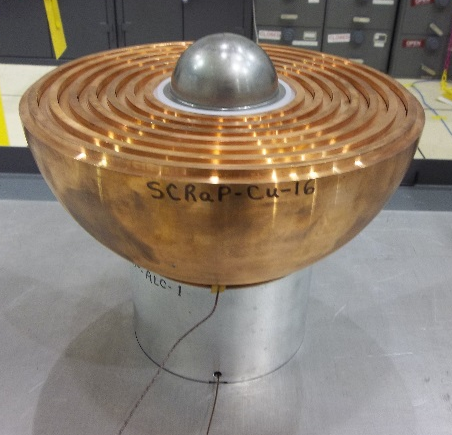
\includegraphics[width=6cm]{images/scrap1}\caption{\label{fig:BeRP-ball-and}SCR$\alpha$P configuration n°15 during
assembly.}
\par\end{centering}
\end{figure}

\begin{figure}

\begin{centering}
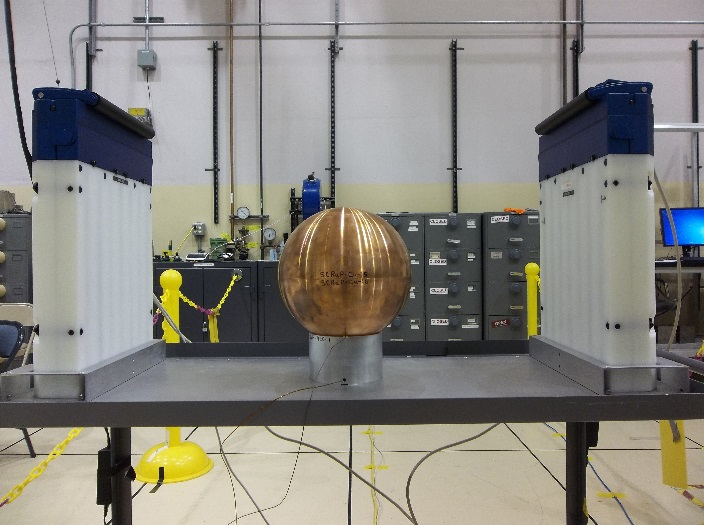
\includegraphics[width=6cm]{images/scrap2}\caption{\label{fig:Experimental-set-up.}Experimental set up. The nuclear
system is surrounded by the NOMAD detectors. }
\par\end{centering}
\end{figure}
 

The general procedure used in this paper for the calculation of NMC
values with the \emph{analog method} is as follow:
\begin{description}
\item [{Step}] 1: A simulation is performed considering both types of neutron
sources (spontaneous fissions and $\left(\alpha-n\right)$ reactions)
and imposing that all histories start (i.e. the instant of the source
event) at t = 0 second. The number of source events to be simulated
must be sufficient for the duration of the desired signal. For each
neutron detection in the two NOMAD detectors, the following information
is recorded: 
\end{description}
\begin{itemize}
\item the type of source from which the neutron originated,
\item the detection time,
\item the history identifier.
\end{itemize}
\begin{description}
\item [{Step}] 2: From the output file is extracted for each type of source
a number of histories corresponding to the desired signal duration
and the intensity of each source.
\item [{Step}] 3: The beginning of each of the histories (and therefore
the corresponding detection times) are modified by sampling from a
uniform random law over the signal duration interval. A modulo function
of parameter the signal duration is applied on each detection time
to confine the detection times to the desired time interval. This
last step is necessary since some histories may start close enough
to the end of the signal so that their detection times can appear
beyond the chosen signal duration. 
\item [{Step}] 4: All detection times are merged to form the final signal. 
\item [{Step}] 5: Other post-processing can be applied to simulate experimental
instrumentation behavior such as the detectors dead-time or the detectors
time resolution. For this present work no experimental instrumentation
effect is taken into account and this step is skipped.
\item [{Step}] 6: NMC values are calculated using post processing programs
as for a signal originating from real detectors.
\end{description}
There is several benefits to this approach for the \emph{analog method}.
First, the simulation of the transport of one history is an independent
process from the transport of other histories. Therefore, this approach
does not necessarily require a parallelized computation code and it
is sufficient to run several instances of the computation code, taking
care to modify the seed of the random generator. Secondly, it is possible
to adjust the parameters used in post-processing (sources intensities,
sources types, signal duration) to build a new signal without having
to recalculate the transport part whose calculation time is much longer
than that of the post-processing part. Another interesting point is
the possibility to change the seed used to sample the beginning time
of the histories (step 3). One can then create multiple signals that
all contain the same knowledge (i.e. fission chains, detections, etc.)
but distributed differently (although the uniform random law is still
used). This allow for the study of statistical properties (expected
mean and standard deviation) of observable calculated from these signals.\textcolor{blue}{{} }

Concerning the \emph{direct method} the post processing program only
needs the result of the first step for the calculation of the two
required terms $p_{N}$ and $pdf(t)$. Since each recorded detection
has been associated to its corresponding history identifier the calculation
of $p_{N}$ is straightforward. The calculation of $pdf(t)$, must
be done taking into account all the combination of detections originating
from a history. It is important that the binning used to calculate
$pdf(t)$ is fine and cover a large time range in order to include
both prompt and delayed neutrons. In the following comparison the
binning is composed of $1000$ values logarithmicaly distributed between
$1\cdot10^{-9}$ and $1\cdot10^{4}$ seconds.

As seen from Equation \ref{eq:y_final}, $Y_{1}(\tau)$, $Y_{2}(\tau)$
and $Y(\tau)$ are link to each other, moreover as no discrepancy
is expected for the single counting rate, this paper focus only on
the comparisons between $Y(\tau)$ and $\mathring{Y}(\tau)$.

According to the SCR$\alpha$P benchmark report \cite{Benchmark Scrap}
neutrons arise from approximately 128500 spontaneous fissions per
second and 4200 $\left(\alpha-n\right)$ reactions per second. The
duration of the simulated signal is about 5500 seconds which approximately
represents $7\cdot10^{8}$ spontaneous fissions and $2.3\cdot10^{7}$$\left(\alpha-n\right)$
reactions. The step 1 has been performed using a modified version
of MORET \cite{MORET} which allows the analog simulation of neutrons
and the record of simulation information into list-mode like files.
A first comparison is presented in Figure \ref{fig:Y-values} for
samples widths from $1\cdot10^{-7}$ to $1\cdot10^{4}$ seconds between
the \emph{direct method} (i.e. $\mathring{Y}(\tau)$) in red and the
\emph{analog method} (i.e. $Y(\tau)$) in blue. For samples width
smaller than $1\cdot10^{-2}$\,seconds both methods are in good agreement,
unfortunately above this samples width the \emph{analog method} start
to exhibit large fluctuations that make the comparison infeasible.
Futures analyses focus on samples widths greater than $1\cdot10^{-2}$\,seconds. 

\begin{figure}
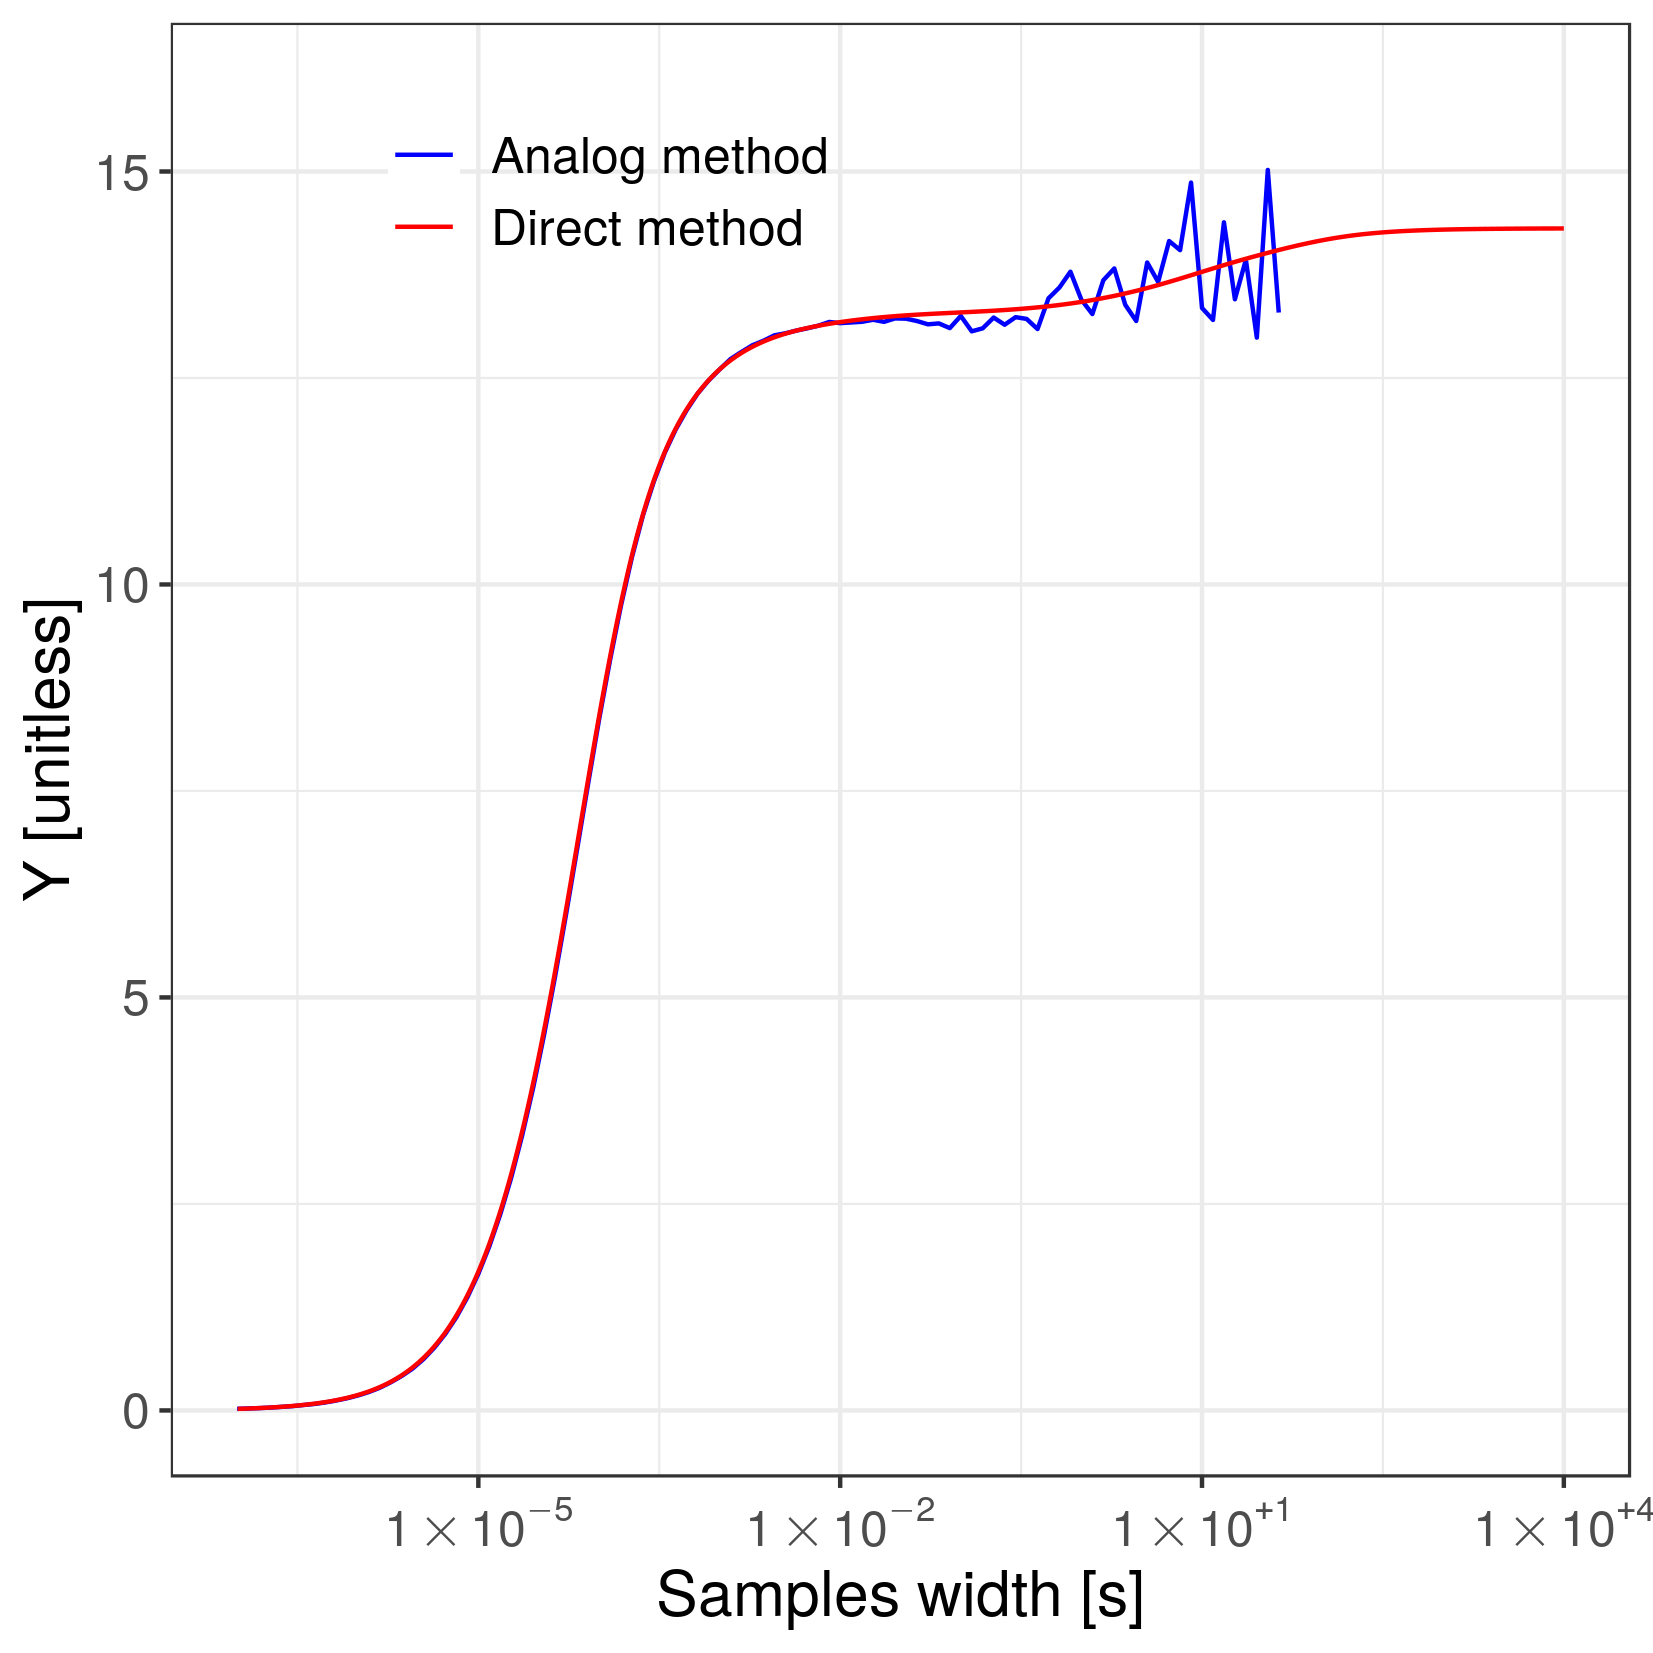
\includegraphics[width=7cm]{images/plot0}\caption{\label{fig:Y-values}Comparison of $Y(\tau)$ and $\mathring{Y}(\tau)$
for samples widths between\, $1\cdot10^{-7}$\,and~$1\cdot10^{4}$~seconds.}
\end{figure}

A naive way to make the comparison feasible for larger samples widths
is to lengthen the simulated signal duration by performing additional
simulations. Unfortunately this would be in practice inaccessible
for desktop computers due to the high CPU time consuming (we are speaking
of orders of magnitude longer simulation duration). Another approach
is to create a number of independent signals by changing the seed
as explained before. With a set of 100 independent generated signals
Figure \ref{fig:Comp_100_signals} show the mean (blue curve) and
the standard deviation (black curve) of $Y(\tau)$ values. From this
figure it can be inferred that the averaged \emph{analog} $Y(\tau)$
values are consistent with the \emph{direct method} up to samples
width of $10$ seconds. This figure also show a very good agreement
between the standard deviation based on {[}10{]} (black cross points)
and based on the set of generated signals. Once again lets recall
that all these signals contains the same ``amount of knowledge''
(i.e. sames histories, detections, etc.).

\begin{figure}
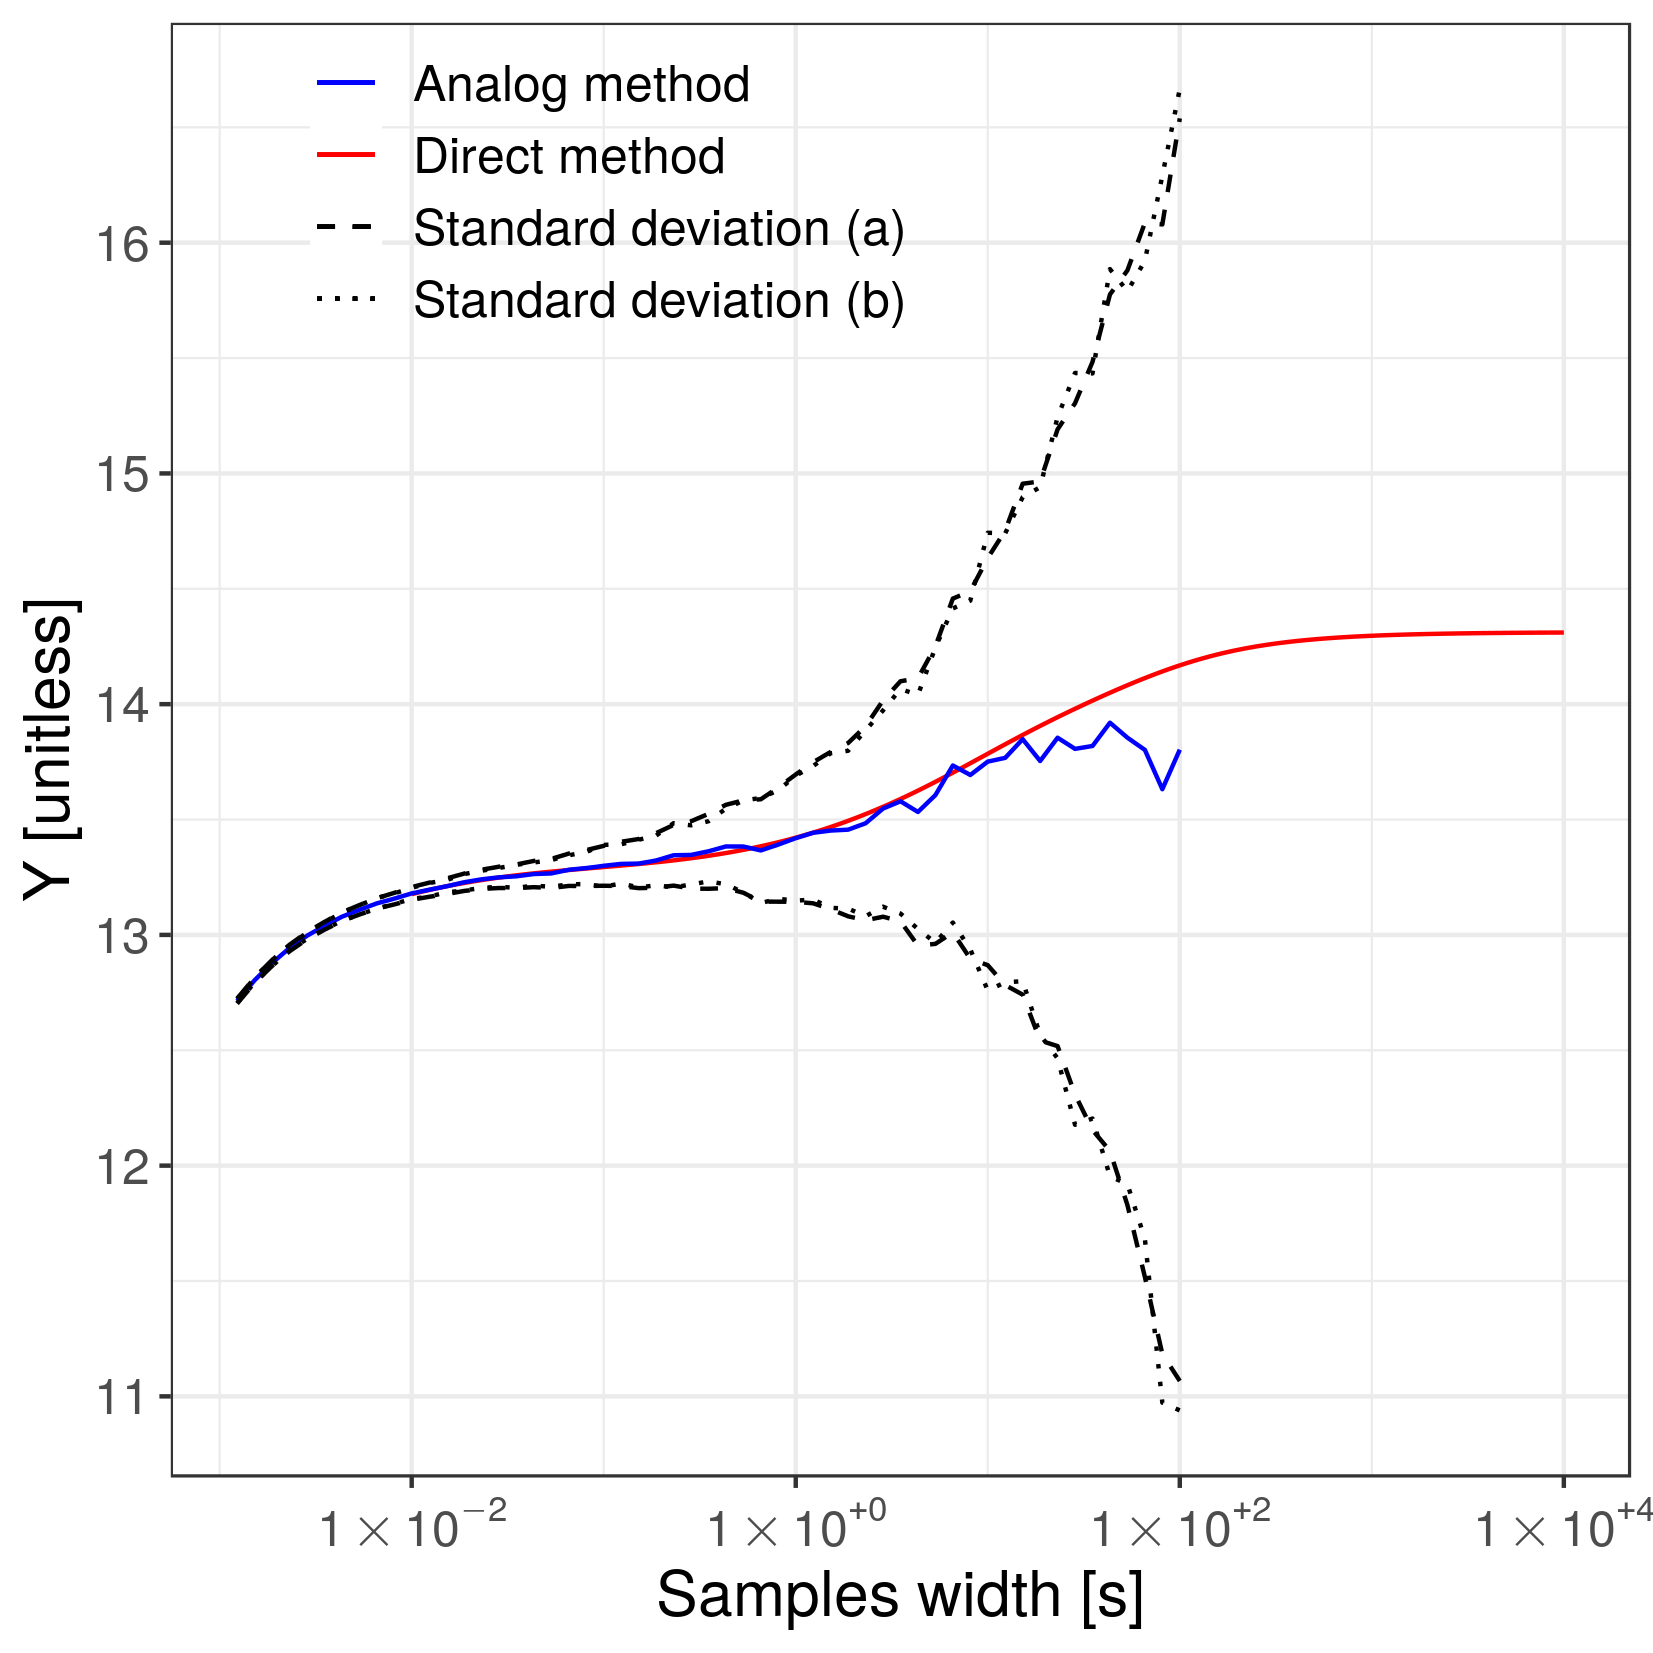
\includegraphics[width=7cm]{images/plot1}\caption{\label{fig:Comp_100_signals}Comparison of $\mathring{Y}(\tau)$ and
averaged $Y(\tau)$ values over 100 generated signals.}
\end{figure}

To go further in the comparison, one may generate additional simulated
signals. Unfortunately as presented in Figure \ref{fig:Comp_1000_signals}
the use of 1000 generated signals (green curve) do not show any significant
improvement compare to the use of 100 generated signals.

\begin{figure}
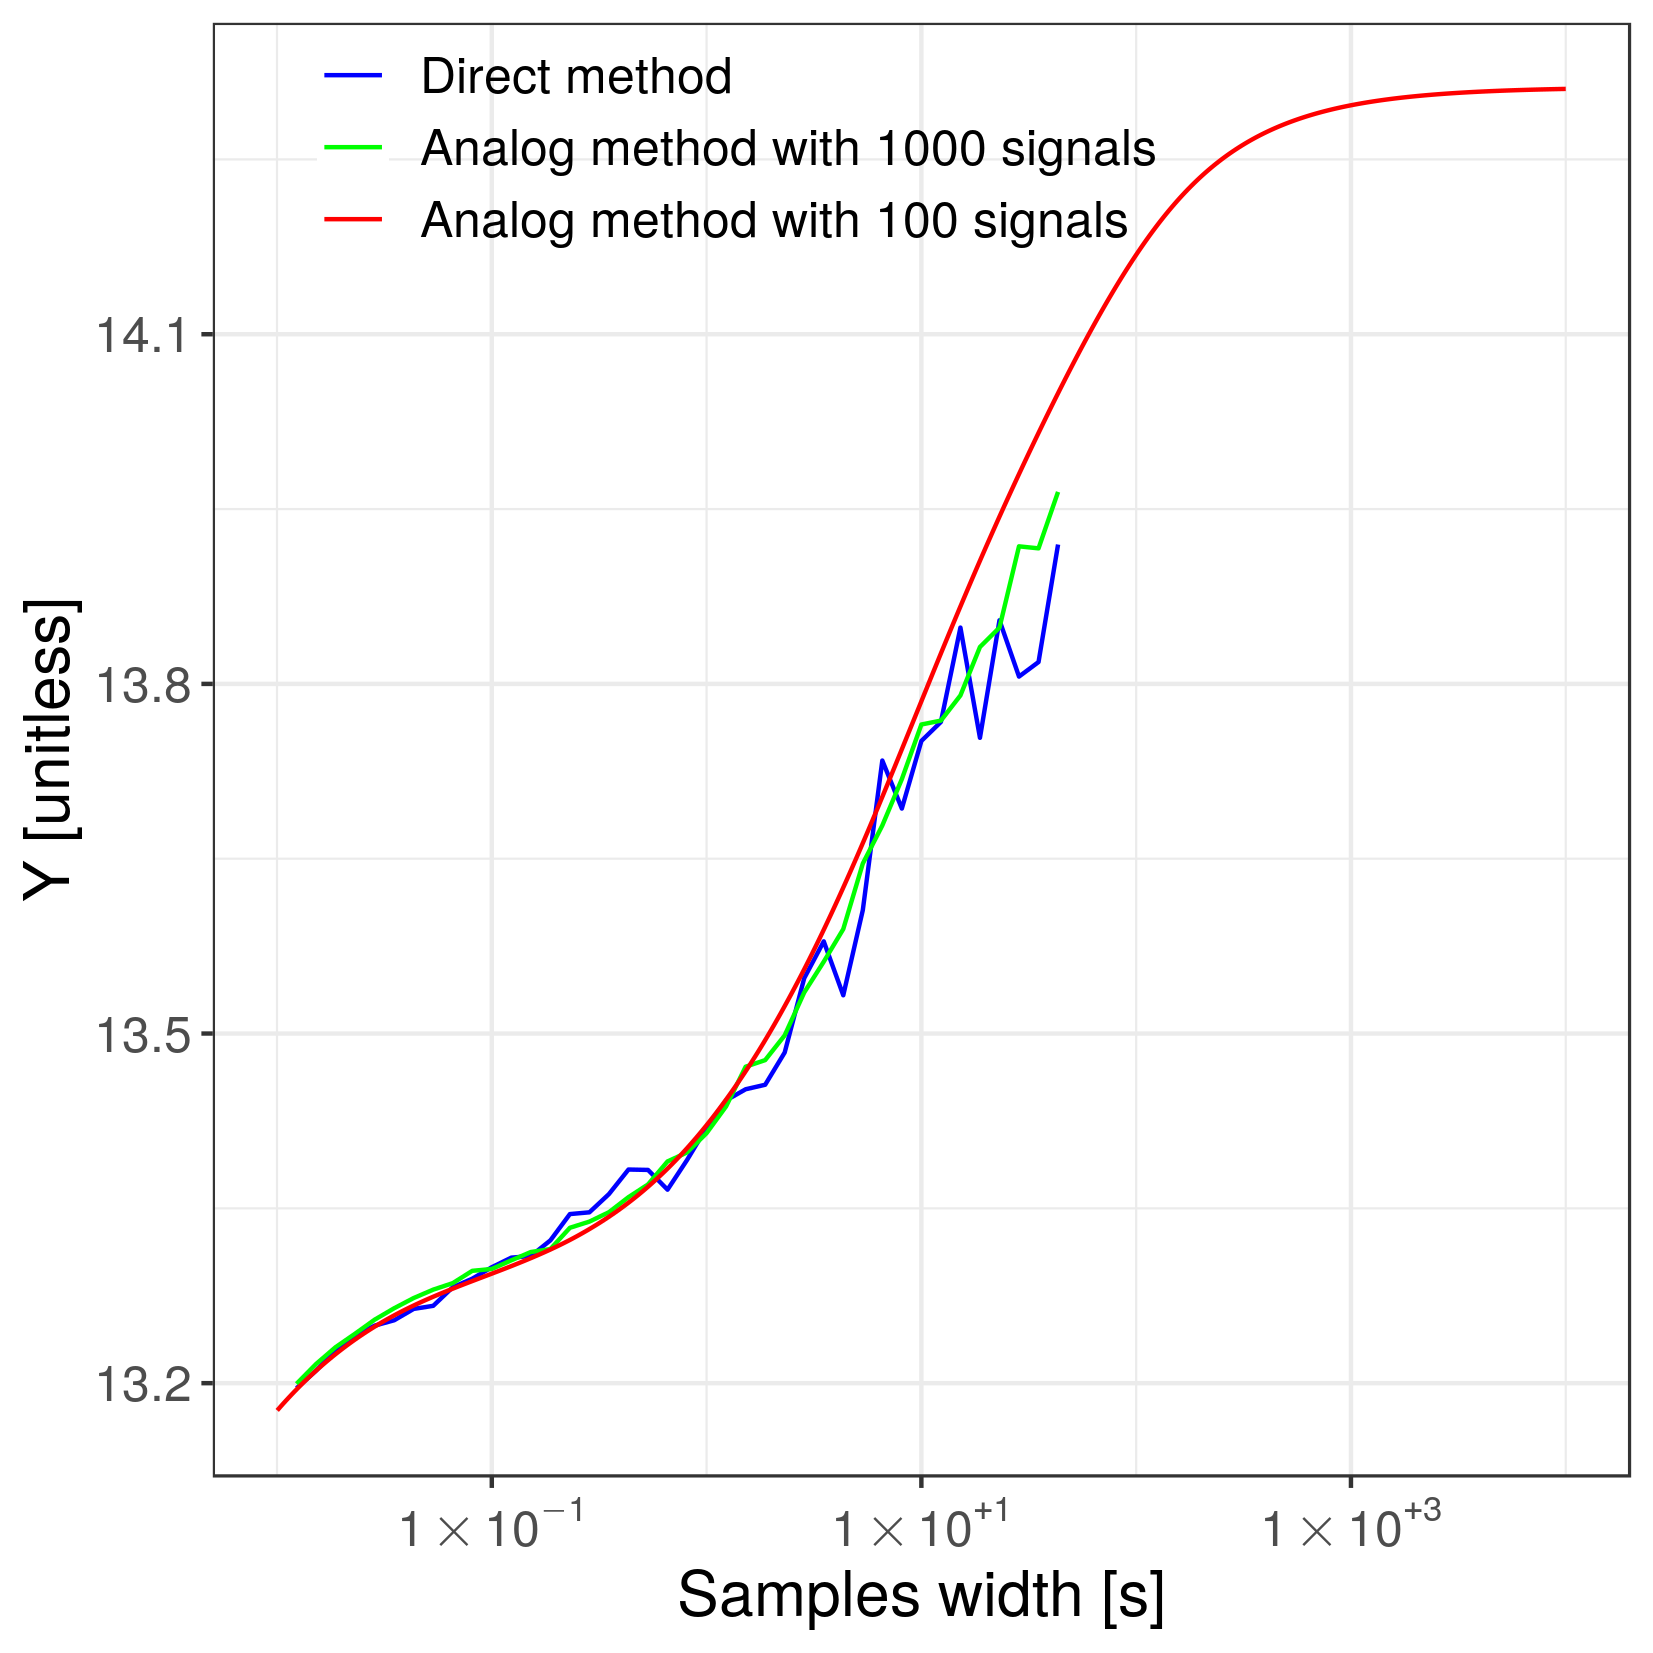
\includegraphics[width=7cm,height=7cm]{images/plot2}

\caption{\label{fig:Comp_1000_signals}Comparison of $\mathring{Y}(\tau)$
and averaged $Y(\tau)$ values over 100 generated signals.}
\end{figure}

Although the previous figures tend to show consistency between the
two methods, the delayed neutron part of the Feynman curve could not
be compared. To access this portion another approach must be used.
By reducing the intensity of the neutron sources it is possible to
artificially lengthen the signal duration for the same number of simulated
histories. It should be noted that this method does not require additional
simulation (neutron transport), as the signal broadening is performed
with post-processing functions. In this way, a new set of 100 signals
have been generated with a duration equal to $5.5\cdot10^{6}$ seconds
(about 64 days) corresponding to a source composed of 128.5 SF per
second and about 4.2 $\left(\alpha-n\right)$ reactions per second.
Results presented in Figure \ref{fig:Comp_long} for samples widths
from $1\cdot10^{-2}$ to $1\cdot10^{4}$ seconds between the direct
method (red curve) and the averaged $Y(\tau)$ values (blue curve)
show a good agreement over all the inspected range.

\begin{figure}
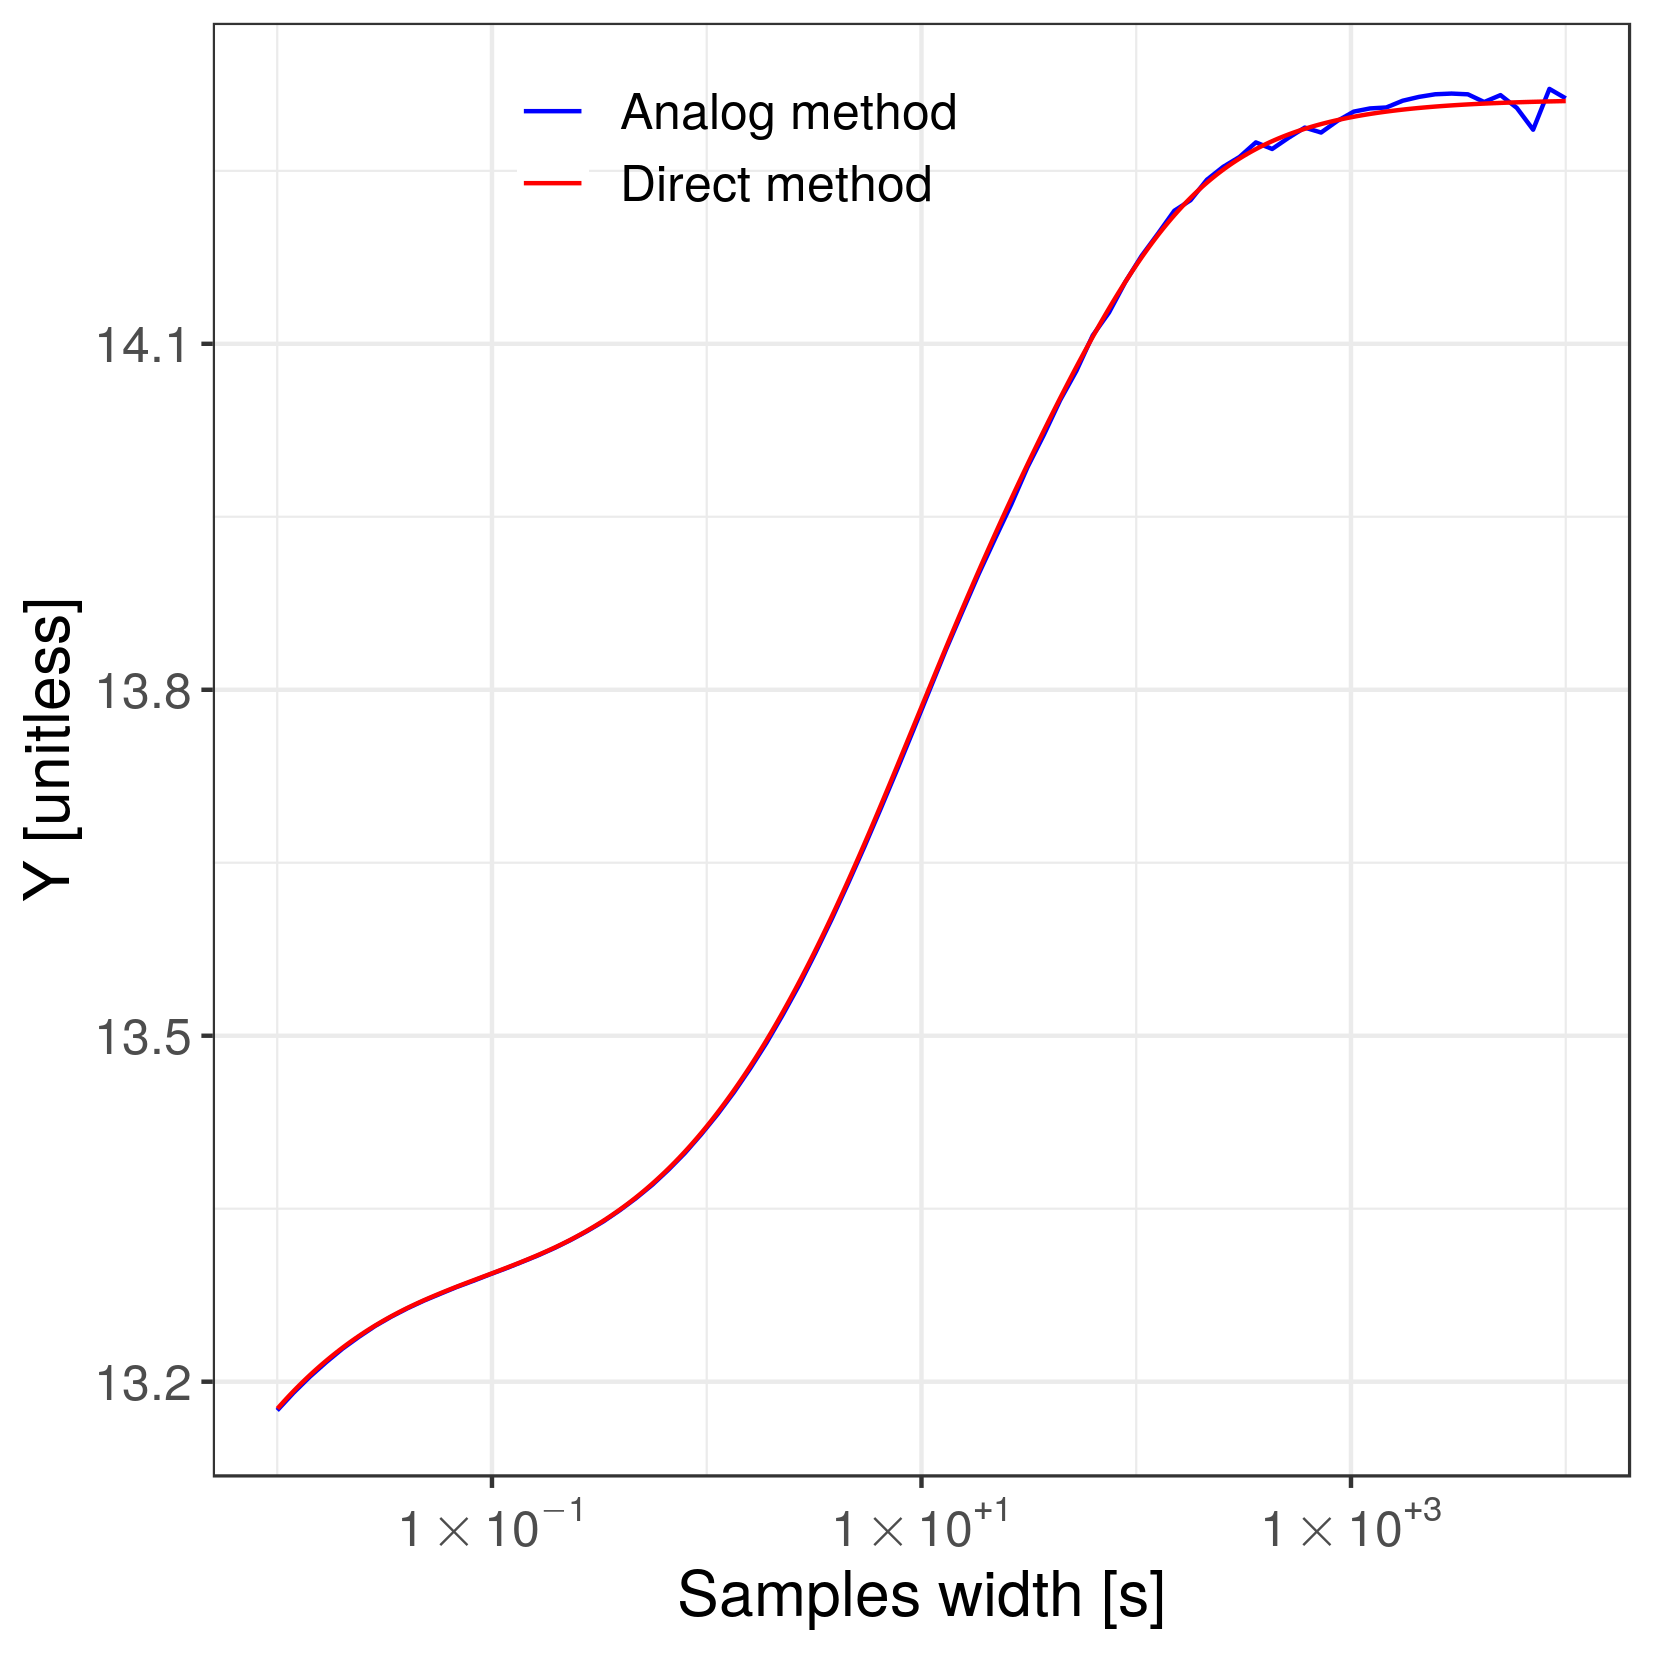
\includegraphics[width=7cm]{images/plot4}\caption{\label{fig:Comp_long}Comparison of $Y(\tau)$ and $\mathring{Y}(\tau)$
based on an extended signal.}
\end{figure}

For the time being, exact formula of the variance of $\mathring{Y}(\tau)$
has not been yet established and estimation of this value is relying
on multiple sets of histories. Figure \ref{fig:Y_var_cmp} shows the
variance as a function of the sets' size express as the proportion
of histories used to calculate $Y$ from the previous plots (\ref{fig:Y-values}
to \ref{fig:Comp_1000_signals}). The samples width is equal to $1\,s$
and each variance value is calculated with 50 sets of histories. The
blue line is a fit demonstrating that the variance varies as the inverse
of the number of simulated histories. This is in contrast with the
\emph{analog method} whose the variance varies with the inverse of
the number of samples. This figure also includes the uncertainty of
$Y(\tau\,=\,1\thinspace s)$ from Figure \ref{fig:Comp_100_signals}
as a red dashed line (with nominal sources intensities and with all
the available histories).

Taking into account that the variance of $Y(\tau=1\thinspace s)$
for the SCR$\alpha$P experiment (Figure \ref{fig:Comp_100_signals})
is about 0.8, this figure shows that the direct method has about the
same variance as the analog method using about 0.1\% of the total
simulated histories. It has to be noted that this gain depends on
many parameters which are not presented here due to the lack of theoretical
formula of the direct method's variance. Nevertheless it is obvious
that this gain increase with the intensity of the signal since the
fission chains tends to overlap more and more.

\begin{figure}
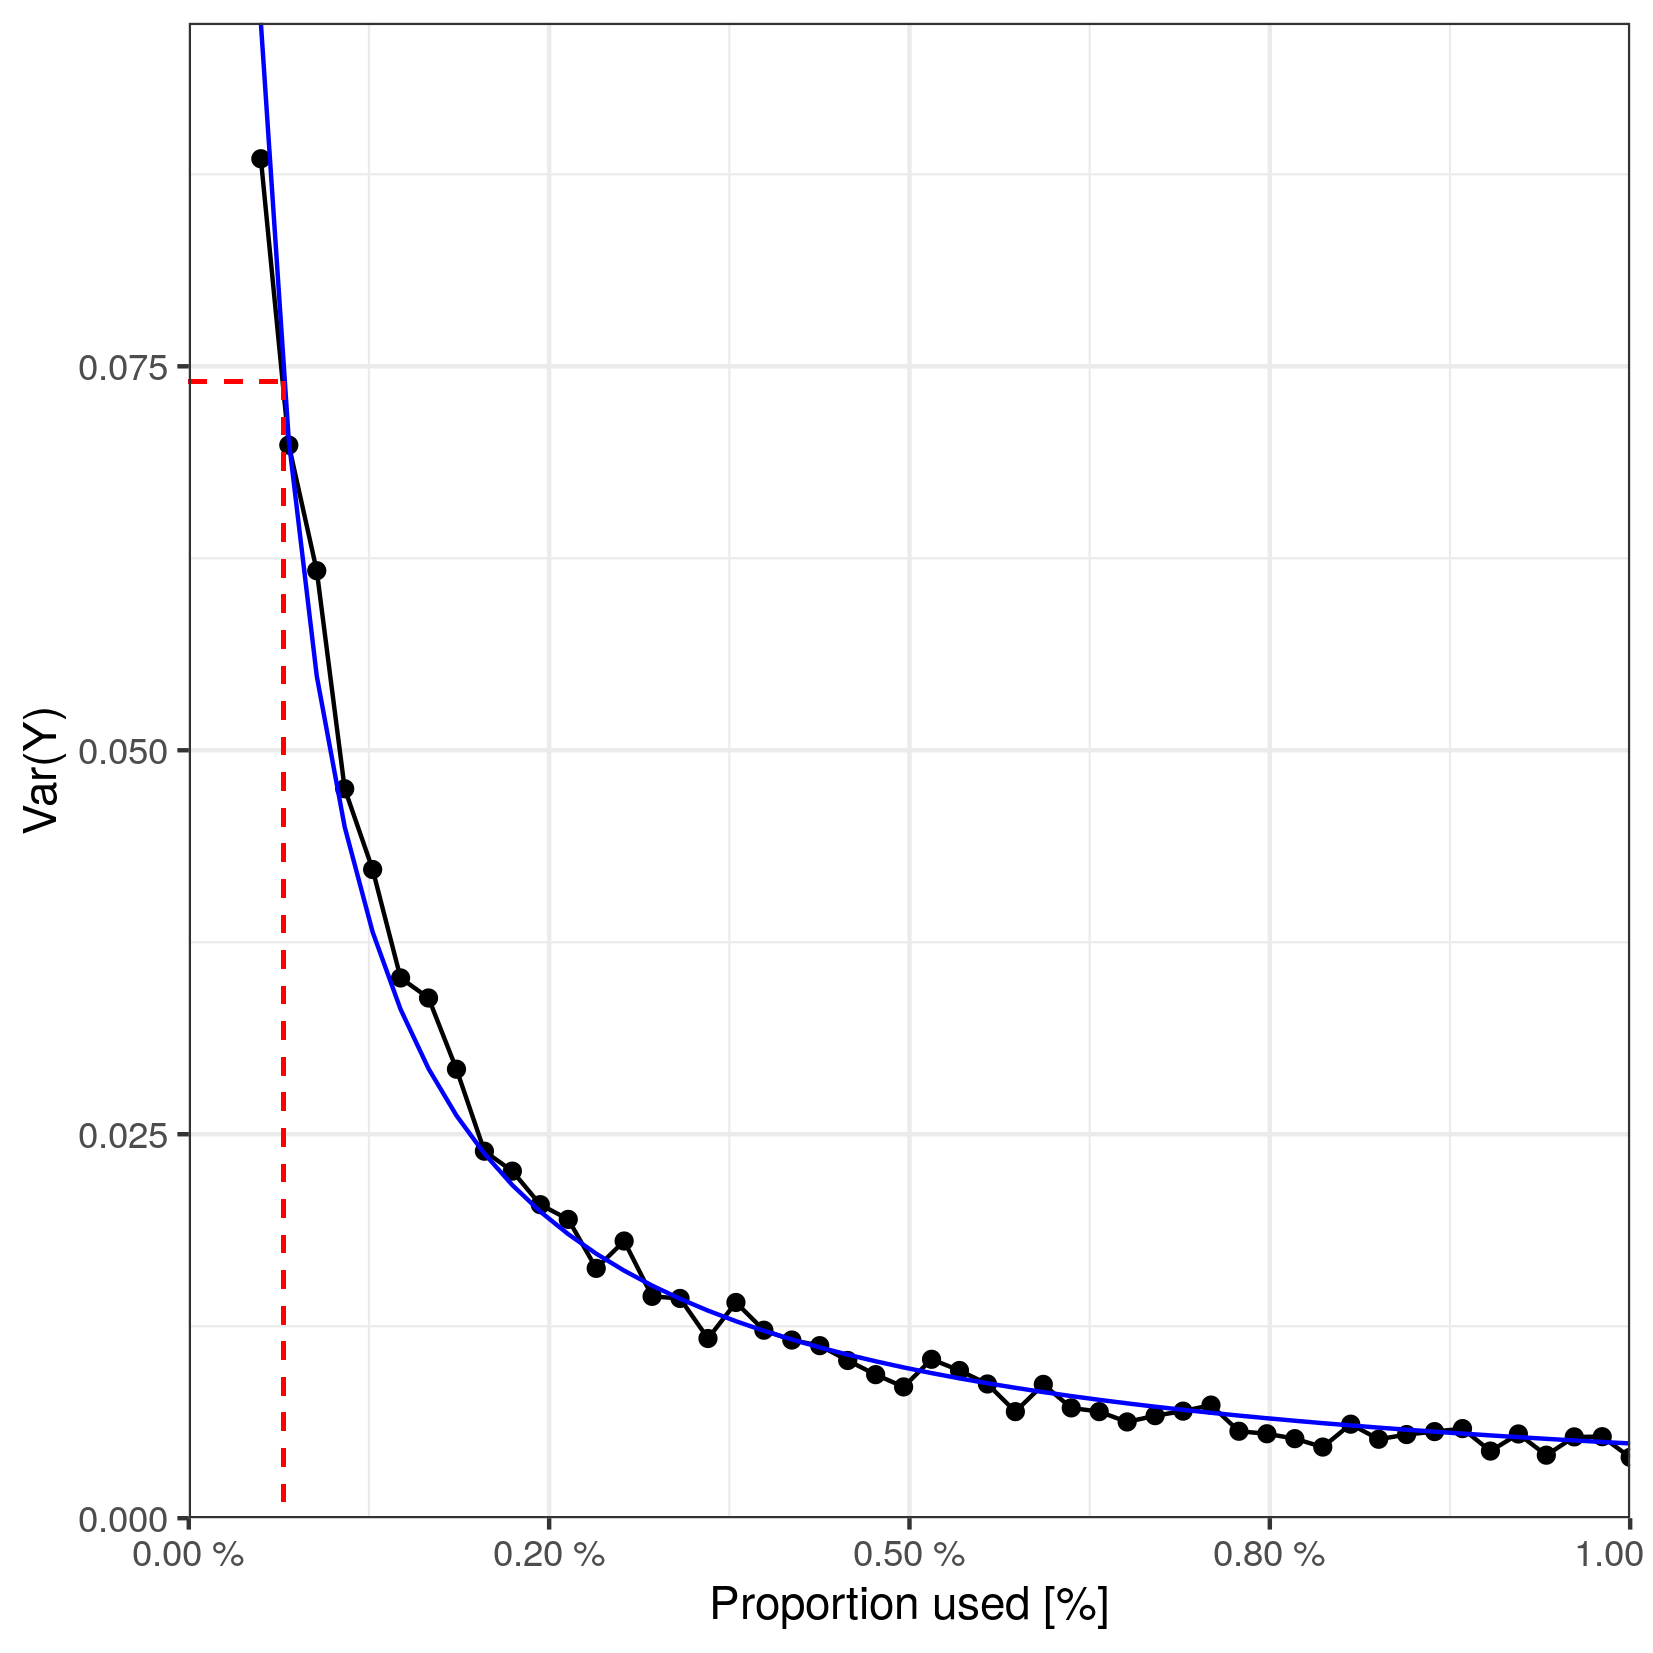
\includegraphics[width=7cm]{images/plot6}\caption{\label{fig:Y_var_cmp}Variance of $\mathring{Y}(\tau)$ as a function
of the proportion of histories used.}
\end{figure}


\section{Conclusion and future work}

Traditionally, NMC values are calculated using similar tools to exploit
the detections obtained by the experiment's detectors or by simulation.
However, in some cases this approach can be very CPU intensive. The
\emph{direct method} uses additional information provided by the simulations
to significantly reduce uncertainties and thus simulation times. However,
as the present situation stands, this method cannot completely replace
the traditional method. The main identified limitations are the following:
\begin{itemize}
\item requirement of sub-critical system in a steady state (i.e. constant
power with time);
\item detector dead time not take into account;
\item higher order of counting rates (triple, etc.) are not yet derive. 
\end{itemize}
Concerning the last point, it should be noted that these values are
often difficult to obtain by simulation due to the need of a high
detection efficiency to keep the variance reasonable. Therefore the
development of the calculation of this value with the \emph{direct
method} could be very advantageous for applications that use these
types of measures.
\begin{thebibliography}{10}
\bibitem{NMC Robba}A.A. Robba, E.J. Dowdy and H.F. Atwater, \textquotedbl Neutron
Multiplication Measurements Using Moments of the Neutron Counting
Distribution\textquotedbl , Nuclear Instruments and Methods 215 (1983)
473-479

\bibitem{Szieberth}M. Szieberth, J.L. Kloosterman, ``New Methods
for the Monte Carlo Simulation of Neutron Noise Experiments in ADS''

\bibitem{Feynman}R. P. FEYNMAN, et. al., ``Dispersion of the Neutron
Emission in U-235 Fission'', J. Nuclear Energy, 1956, Vol. 3, pp.
64 to 69. Pergamon Press Ltd., London

\bibitem{Uhrig}R. UHRIG, ``Random Noise Techniques in Nuclear Reactor
Systems'', John Wiley \& Sons Inc, 1970

\bibitem{Hutchinson1}J. HUTCHINSON, et. al., ``Subcritical Multiplication
experiments \& Simulations: Overview and Recent Advances,'' ANS Advances
in Nonproliferation Technology and Policy Conference, Santa Fe NM,
September 2016.

\bibitem{Cifarelli}D.Cifarelli, W. Hage, “Models for a Three-Parameter
Analysis of Neutron Signal Correlation Measurements for Fissile Material
Assay,” Nuc. Instr. Meth. A251, 550-563, 1986.

\bibitem{SCRaP}J. HUTCHINSON, et. al., ''Subcritical Copper-Reflected
α-phase Plutonium (SCRαP) Measurements and Simulations'', Los Alamos
Report LA-UR-17-XXXX, 2017

\bibitem{MORET}B. COCHET, et. al. ``Capabilities overview of the
MORET 5 Monte Carlo code'', Joint International Conference on Supercomputing
in Nuclear Applications and Monte Carlo 2013 (SNA + MC 2013), La Cité
des Sciences et de l'Industrie, Paris, France, October 27-31, 2013.

\bibitem{Benchmark Scrap}Benchmark SCRaP

\bibitem{Uncertainties on Y}Smith-Nelson, et. al. ``Uncertainties
of the Yn Parameters of the Hage-Cifarelli Formalism'', Los Alamos
Report LA-UR-15-21365, 2015.
\end{thebibliography}

\end{document}
